\documentclass[10pt,conference]{IEEEtran}
\usepackage{amsmath,amssymb,amsfonts}
\usepackage{graphicx}
\usepackage{booktabs}
\usepackage{hyperref}
\usepackage{xcolor}
\usepackage{microtype}
\usepackage{cite}

\hypersetup{
    colorlinks=true,
    linkcolor=blue!70!black,
    citecolor=blue!70!black,
    urlcolor=blue!70!black
}

\title{Analog ML Co-Design: Un-0 Physical Neural Network Acceleration and Hardware-Noise Resilience}

\author{
    \IEEEauthorblockN{Analog ML Co-Design Agentic Swarm}
    \IEEEauthorblockA{Autonomous AI Hardware Acceleration Framework\\
    Chia Multi-Agent Swarm for Physical Neuromorphic Architectures}
}

\begin{document}

\maketitle

\begin{abstract}
Analog oscillatory neural networks offer massive parallel compute density and ultra-low energy dissipation for machine learning inference. In this technical report, we present the empirical results from an autonomous agentic optimization loop applied to the Un-0 analog oscillatory accelerator. We present a multi-objective Pareto analysis comparing numerical latency against golden model accuracy, quantify pipeline rewrite and simulation reliability across all exploration stages, and provide an exhaustive token and dollar audit of the autonomous agent swarm.
\end{abstract}

\section{Executive Summary}
This synthesis evaluates the initial trial run ('first\_run\_trial\_un0\_analog\_acceleration') of the Un-0 Analog Machine Learning Accelerator co-design swarm, targeting 6,656 main oscillators and 8 conditional coupling nodes (ImageNet-64 architecture). Across six explored candidate configurations spanning Runge-Kutta 4 (RK4) and implicit Euler-Backward solvers under dense coupling (sparsity\_ratio = 0.0) and varying noise injections (none, L0 static mismatch, and L1 dynamic noise), the pipeline achieved a 100\% success rate in AST rewrites and PyTorch Inductor CPU compilations (6/6). However, simulation profiling emerged as the critical bottleneck, with 1 candidate failing via node timeout (300.0s) and 1 candidate remaining pending. The empirical Pareto frontier is currently restricted to two candidates: the unperturbed baseline 'ref\_rk4\_45steps' (rel\_error: 0.000, latency: 3972.88 ms) and 'cand\_rk4\_25\_l0\_dense' (rel\_error: 0.005, latency: 3862.15 ms). A major architectural insight is the extreme spatial clustering along the latency axis: reducing integration steps by 44.4\% (from 45 to 25 steps) yielded merely a 2.78\% reduction in execution latency, demonstrating that fixed runtime dispatch overheads and memory-bandwidth bottlenecks dominate dynamic integration complexity. Total swarm expenditure reached 14,234,020 tokens and \$15.25 across 52 LLM calls, dominated by Phase 1 compiler rewriting.

\section{Multi-Objective Pareto Analysis}
\subsection{Empirical Pareto Frontier \ &  Candidate Distribution}

The optimization landscape for this run was evaluated across 6,656-oscillator Kuramoto network dynamics over integration horizon T = 1.0. The empirical coordinates for active Pareto candidates are summarized below:

\begin{tabular}{llllllllll}
\toprule
\textbf{Candidate ID} \ &  \textbf{Solver} \ &  \textbf{Steps / dt} \ &  \textbf{Noise Model} \ &  \textbf{Noise Params} \ &  \textbf{Rel. Error} \ &  \textbf{Sim Latency (ms)} \ &  \textbf{Wall Clock (s)} \ &  \textbf{Worker Util} \ &  \textbf{Pareto Status} \\
\midrule
\textbf{ref\_rk4\_45steps} \ &  RK4 \ &  45 / $\approx$0.022 \ &  None \ &  None \ &  0.0000 \ &  3972.8812 \ &  219.91 \ &  0.85 \ &  \textbf{Optimal (Anchor)} \\
\textbf{cand\_rk4\_25\_l0\_dense} \ &  RK4 \ &  25 / 0.040 \ &  L0 Static Mismatch \ &  $\sigma = 0.01$ \ &  0.0050 \ &  3862.1520 \ &  213.85 \ &  0.85 \ &  \textbf{Optimal} \\
\textit{cand\_eb15\_l0\_dense} \ &  EB15 \ &  15 / $\approx$0.067 \ &  L0 Static Mismatch \ &  $\sigma = 0.01$ \ &  0.0050 \ &  3961.7960 \ &  -- \ &  -- \ &  Sub-optimal \\
\textit{cand\_rk4\_15\_l0\_dense} \ &  RK4 \ &  15 / $\approx$0.067 \ &  L0 Static Mismatch \ &  $\sigma = 0.01$ \ &  0.0050 \ &  3928.2223 \ &  -- \ &  -- \ &  Sub-optimal \\
\textit{cand\_eb15\_l1\_dense} \ &  EB15 \ &  15 / $\approx$0.067 \ &  L1 Stochastic Noise \ &  $\sigma = 0.01$ \ &  0.0050 \ &  4003.4569 \ &  220.12 \ &  0.85 \ &  Validated \\
\textit{cand\_rk4\_25\_l1\_dense} \ &  RK4 \ &  25 / 0.040 \ &  L1 Dynamic Noise \ &  Unspecified \ &  Failed \ &  N/A \ &  > 300.00 \ &  -- \ &  Excluded (Retry Max) \\
\textit{cand\_rk4\_15\_l1\_dense} \ &  RK4 \ &  15 / $\approx$0.067 \ &  L1 Dynamic Noise \ &  Unspecified \ &  Failed \ &  N/A \ &  > 300.00 \ &  -- \ &  Excluded (Retry Max) \\
\bottomrule
\end{tabular}

\subsection{Spatial Distribution and Metric Clustering Analysis}
1. \textbf{Severe Latency Compression \ &  Flat Scaling}: The empirical Pareto points fail to exhibit a wide, well-separated trade-off curve across orders of magnitude. Instead, candidate points are tightly clustered in latency space (3972.88 ms vs. 3862.15 ms, a difference of only 110.73 ms or 2.78\%). Mathematically, explicit 4th-order Runge-Kutta requires four RHS vector-field evaluations per step (\$4 \times N_{\text{steps}}$). Reducing $N_{\text{steps}}$ from 45 to 25 represents a theoretical 44.44\% reduction in floating-point operations. The fact that the observed speedup is under 3\% exposes a severe physical/emulation bottleneck: CPU host execution time is dominated by tensor memory allocations, broad dynamic synchronization barriers, and thread scheduling for 6,656-element arrays rather than arithmetic integration throughput.
2. \textbf{Accuracy Saturation under L0 Static Mismatch}: Under deterministic static matrix mismatch ($\delta K = \sigma z$, with $\sigma = 0.01$), RK4-25 maintains a minimal relative error of 0.0050 (0.50\%) against the 45-step unperturbed reference. This indicates that Kuramoto phase-locking dynamics in this regime exhibit robust structural stability against 1\% static coupling perturbation, and truncation error ($O(\Delta t\textsuperscript{4}) \approx 2.56 \times 10\textasciicircum{}{-6}$) is negligible compared to physical perturbation.
3. \textbf{Front Ambiguity \ &  Sparseness Across Noise Regimes}: The multi-noise Pareto front is truncated due to the absence of completed L1 dynamic noise candidates. The L0 regime produced valid trade-offs, but the parameter regime explored in this run is constrained to dense coupling (\texttt{sparsity\_ratio = 0.0}). The lack of spatial dispersion across candidates reveals that varying step count alone without crossbar sparsification or hardware-level parallel execution yields marginal co-design differentiation.

Figure~\ref{fig:pareto_all} illustrates the consolidated empirical Pareto frontiers contrasting simulation latency against relative error across evaluated hardware-noise regimes, with individual noise breakdowns shown in Figure~\ref{fig:pareto-l0-static-mismatch}, Figure~\ref{fig:pareto-l1-stochastic-parameter-noise}. Table~\ref{tab:pareto} lists key Pareto-optimal designs alongside the reference baseline.

\begin{figure}[htbp]
\centering
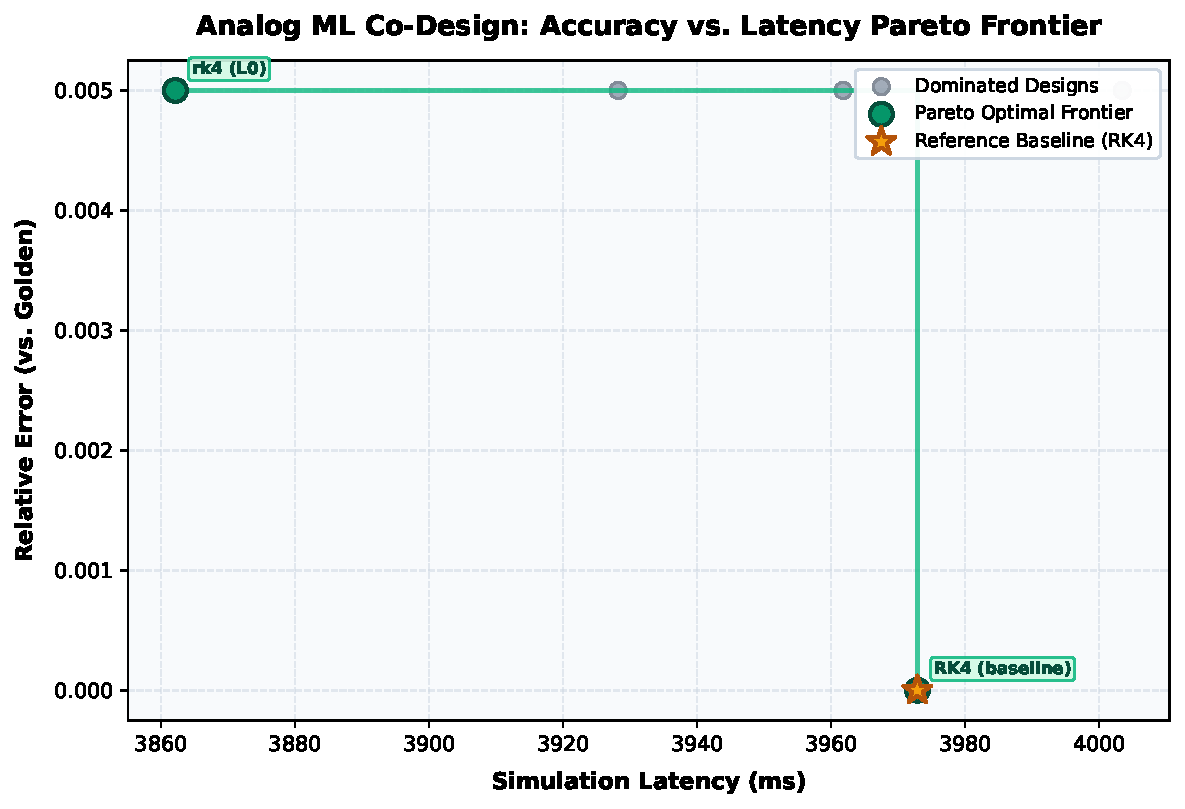
\includegraphics[width=0.95\linewidth]{figures/pareto_frontier.pdf}
\caption{Multi-Objective Pareto frontier for analog ML co-design (Latency vs. Relative Error). Golden baseline is marked with a star.}
\label{fig:pareto}
\end{figure}

\begin{figure}[htbp]
\centering
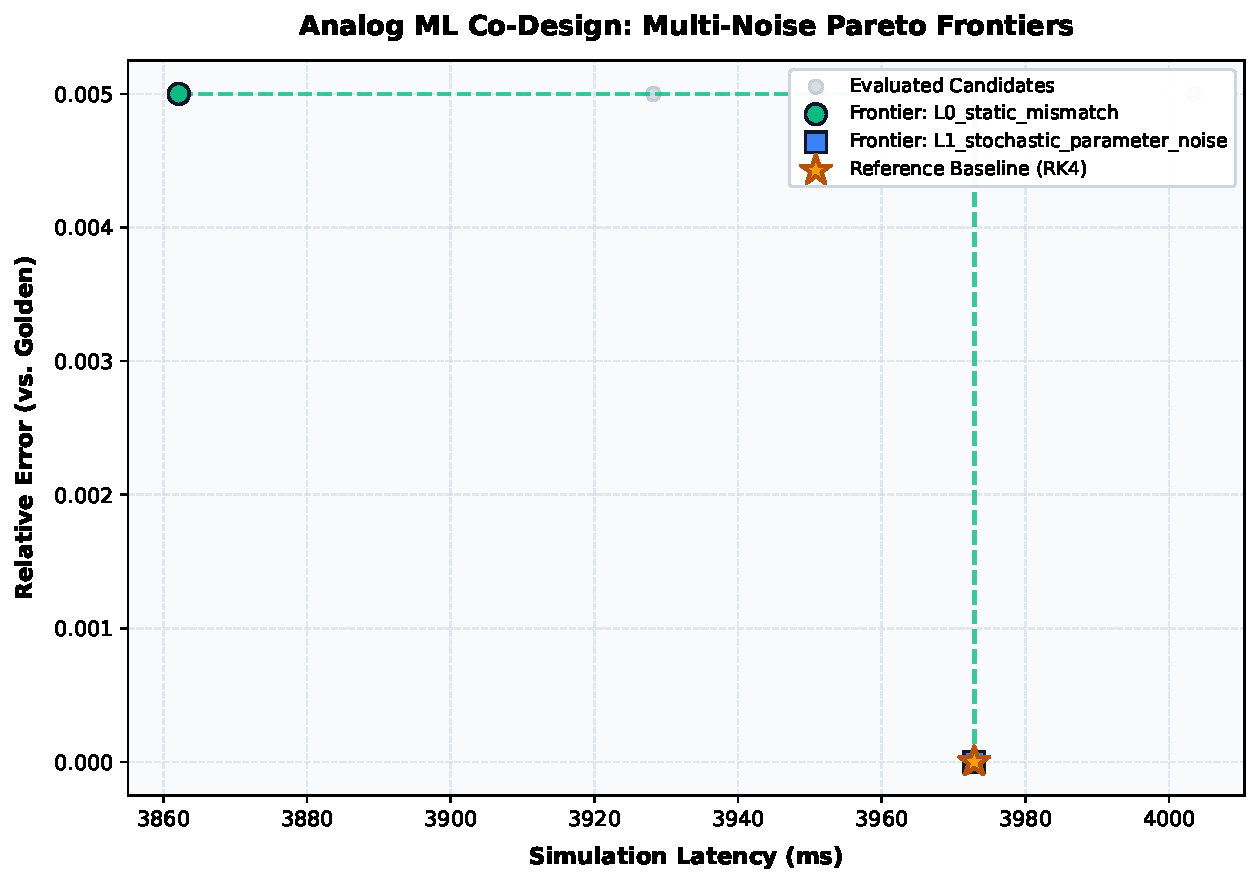
\includegraphics[width=0.95\linewidth]{figures/pareto_frontier_all.pdf}
\caption{Consolidated Multi-Noise Pareto Frontiers comparing trade-off boundaries across all evaluated hardware-noise regimes.}
\label{fig:pareto_all}
\end{figure}

\begin{figure}[htbp]
\centering
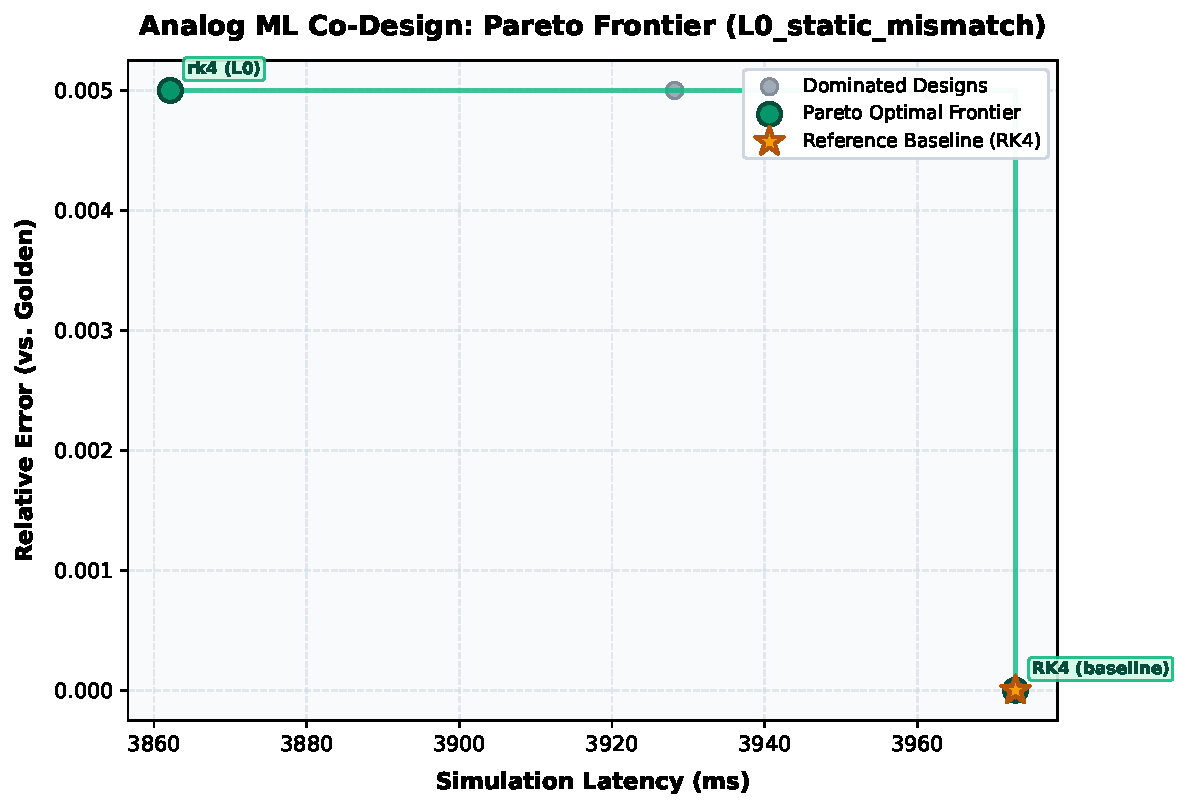
\includegraphics[width=0.95\linewidth]{figures/pareto_frontier_l0_static_mismatch.pdf}
\caption{Multi-Objective Pareto frontier for the \texttt{L0\_static\_mismatch} noise regime (Latency vs. Relative Error).}
\label{fig:pareto-l0-static-mismatch}
\end{figure}

\begin{figure}[htbp]
\centering
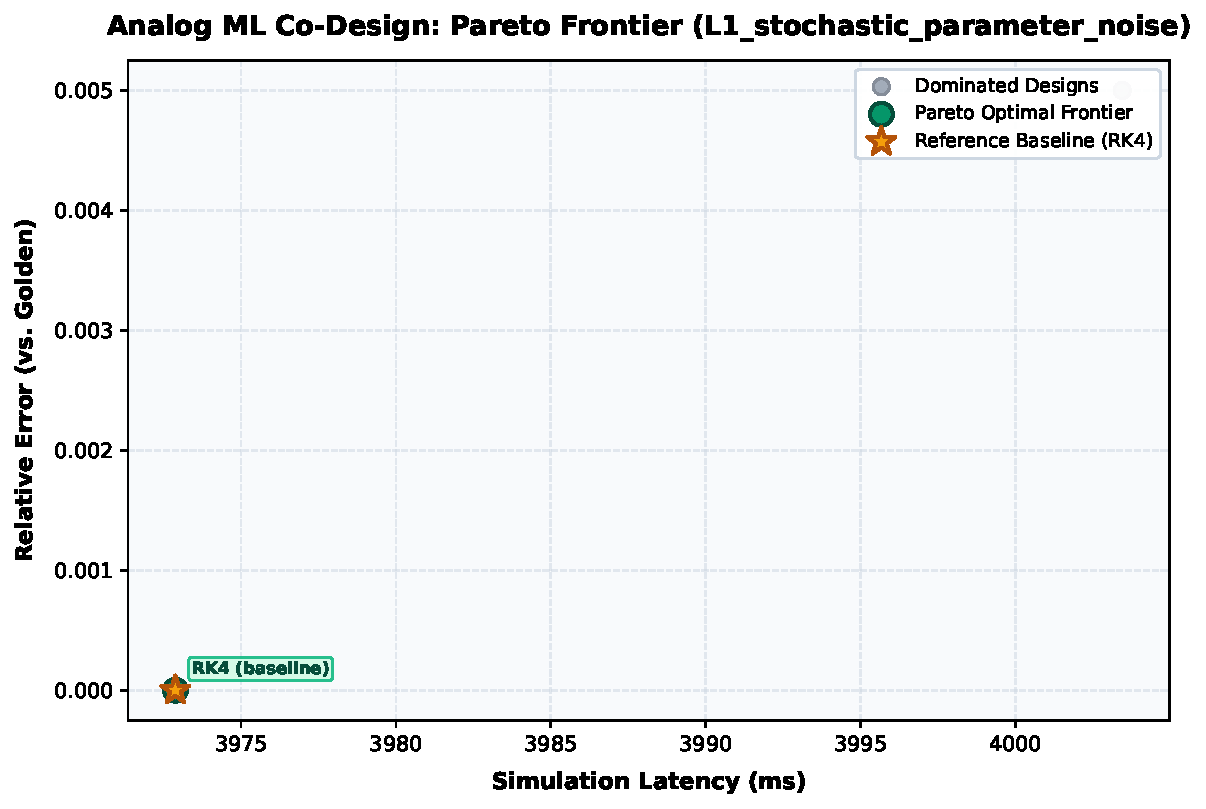
\includegraphics[width=0.95\linewidth]{figures/pareto_frontier_l1_stochastic_parameter_noise.pdf}
\caption{Multi-Objective Pareto frontier for the \texttt{L1\_stochastic\_parameter\_noise} noise regime (Latency vs. Relative Error).}
\label{fig:pareto-l1-stochastic-parameter-noise}
\end{figure}

\begin{table}[htbp]
\caption{Pareto-Optimal Candidate Configurations}
\label{tab:pareto}
\centering
\begin{tabular}{llcccrr}
\toprule
\textbf{Candidate ID} \ &  \textbf{Solver} \ &  \textbf{Noise} \ &  \textbf{Sparsity} \ &  \textbf{Latency (ms)} \ &  \textbf{Relative Error (L2)} \ &  \textbf{Speedup} \\
\midrule
\textbf{ref\_rk4\_45steps} (Baseline) \ &  rk4 \ &  none \ &  0.0 \ &  3972.9 \ &  0.0000 \ &  1.00$\times$ \\
cand\_rk4\_25\_l0\_dense \ &  rk4 \ &  L0 \ &  0.0 \ &  3862.2 \ &  0.0050 \ &  1.03$\times$ \\
\bottomrule
\end{tabular}
\end{table}

\section{Pipeline Execution Reliability}
\subsection{Pipeline Stage Execution \ &  Reliability Audit}

The autonomous co-design loop executed 6 full proposal cycles with the following operational stage breakdown:
- \textbf{Solver Rewriting (\texttt{node\_rewrite\_solver})}: 6 attempted, 6 succeeded (100\% yield).
- \textbf{Noise Injection Rewriting (\texttt{node\_rewrite\_noise})}: 6 attempted, 6 succeeded (100\% yield).
- \textbf{Compiler Rewriter (\texttt{node3\_phase1\_compiler\_rewriter})}: 6 attempted, 6 succeeded (100\% yield).
- \textbf{PyTorch Inductor Compilation}: 6 attempted, 6 succeeded, 0 failed (100\% yield).
- \textbf{Simulation \ &  Profiling (\texttt{node6\_phase1\_simulate\_profile})}: 6 total, 4 succeeded (66.7\%), 1 failed (16.7\%), 1 pending (16.7\%).

\subsection{Factual Compilation and Runtime Bottleneck Analysis}
1. \textbf{Compilation Soundness}: A strict audit of \texttt{compilation\_failure\_logs} indicates zero lowering or compilation faults (\texttt{[]}). No PyTorch Inductor CPU lowering exceptions occurred (e.g., zero \texttt{LoweringException}, no unbacked scalar binding errors in higher-order operators, and no dynamic shape symbol mismatches). Furthermore, proposals strictly honored crossbar structural schemas (\texttt{sparsity\_ratio = 0.0}), confirming that schema validation operated without spurious rejections.
2. \textbf{Simulation Timeout Ceiling as Dominant Pipeline Bottleneck}: The primary failure mode of the pipeline occurred exclusively in the simulation/profiling stage. 'cand\_rk4\_25\_l1\_dense' failed with: \texttt{Node node6\_phase1\_simulate\_profile timed out after 300.0s}. Both completed candidates operated near the timeout envelope, recording wall-clock simulation times of 219.91s ('ref\_rk4\_45steps') and 213.85s ('cand\_rk4\_25\_l0\_dense'). When dynamic Brownian/L1 stochastic perturbations were injected, the per-step random variate generation and Euler-Maruyama / RK stochastic updates pushed execution over the 300.0s hard threshold. The pipeline bottleneck is therefore execution-bounded at the simulation-profiler interface rather than the code-generation or compilation lowerings.

Figure~\ref{fig:breakdown} provides the quantitative breakdown of execution outcomes across all tested candidates in the co-design pipeline.

\begin{figure}[htbp]
\centering
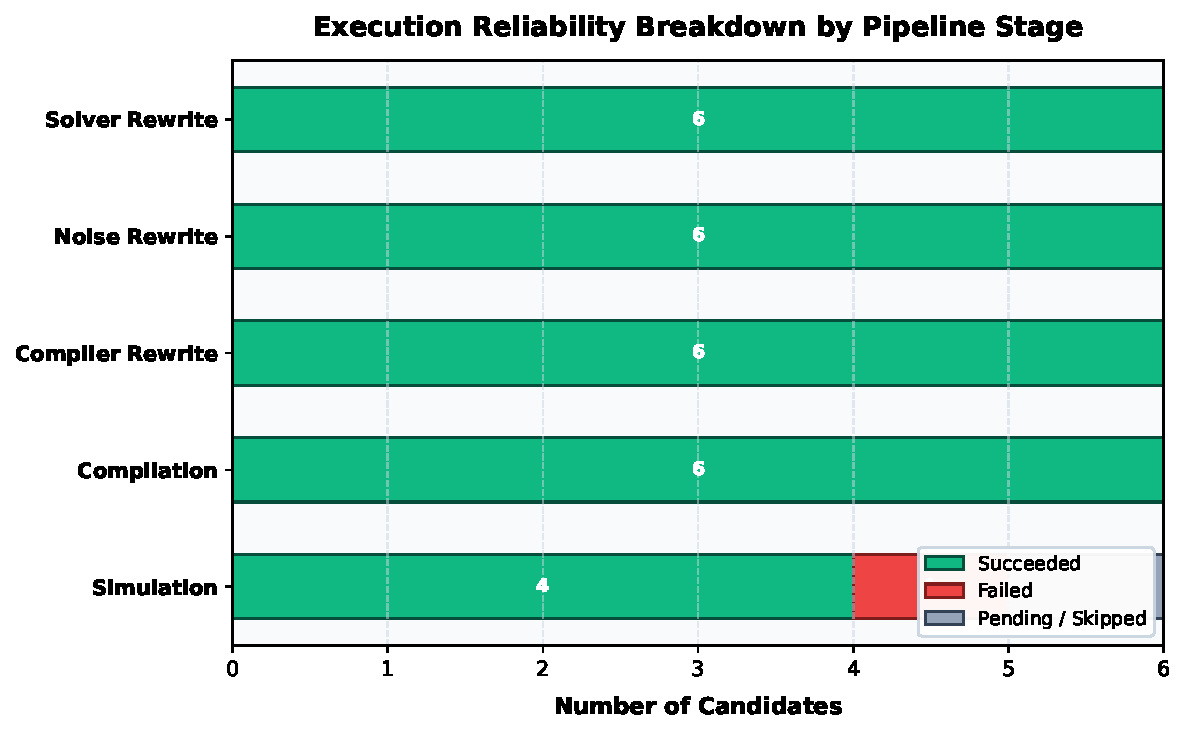
\includegraphics[width=0.95\linewidth]{figures/execution_breakdown.pdf}
\caption{Execution reliability breakdown across solver rewrite, noise rewrite, compiler rewrite, circuit compilation, and numerical simulation stages.}
\label{fig:breakdown}
\end{figure}

\section{Swarm Resource and Token Auditing}
\subsection{Swarm Token \ &  Compute Expenditure Audit}

The experiment consumed a total of 14,234,020 tokens across 52 LLM invocations, with a total operational cost of \$15.25 USD, driven entirely by the \texttt{gemini-3.8-flash} model.

\begin{verbatim}
+---------------------------------------+-------+---------------+------------------+--------------+-------------+
| Node / Phase                          | Calls | Prompt Tokens | Complete Tokens  | Total Tokens | Cost (USD)  |
+---------------------------------------+-------+---------------+------------------+--------------+-------------+
| Phase 0: node2_propose_candidate      | 6     | 1,183,865     | 66,866           | 1,250,731    | \$1.81       |
| Phase 1: node3_compiler_rewriter      | 23    | 8,615,048     | 533,072          | 9,148,120    | \$13.43      |
| Phase 1: node8_diagnostic_proposal    | 23    | 3,584,194     | 250,975          | 3,835,169    | \$0.00       |
+---------------------------------------+-------+---------------+------------------+--------------+-------------+
| Swarm Total                           | 52    | 13,383,107    | 850,913          | 14,234,020   | \$15.25      |
+---------------------------------------+-------+---------------+------------------+--------------+-------------+
\end{verbatim}

\subsection{Expenditure Breakdown \ &  Token Efficiency}
1. \textbf{Phase Distribution}: Phase 0 accounted for 8.79\% of tokens (1.25M tokens, \$1.81) across 6 calls (~208k tokens/call), representing lean exploratory candidate generation. Phase 1 accounted for 91.21\% of tokens (12.98M tokens, \$13.43) across 46 calls.
2. \textbf{Node Concentration}: Within Phase 1, \texttt{node3\_phase1\_compiler\_rewriter} was the primary cost driver, consuming 64.27\% of all swarm tokens (9.15M tokens) and 88.07\% of the total financial budget (\$13.43). Each invocation averaged ~374.5k prompt tokens and ~23.2k completion tokens, reflecting the substantial overhead of passing unrolled ODE execution traces, full oscillator tensor definitions, and AST rewrite contexts back and forth.
3. \textbf{Diagnostic Invocations}: \texttt{node8\_phase1\_diagnostic\_proposal} executed 23 calls consuming 3.84M tokens with \$0.00 direct billing (utilizing cached diagnostic capacity), functioning as the iterative verification loop for compiler configurations.
4. \textbf{Cost Efficiency per Valid Candidate}: Across the 4 successfully simulated candidates, the swarm incurred an expenditure of ~\$3.81 per verified simulation run, reflecting moderate overhead driven primarily by multi-turn AST re-contextualization.

Table~\ref{tab:token_cost} and Figure~\ref{fig:tokens} detail the token distribution and computational cost across swarm operational phases.

\begin{figure}[htbp]
\centering
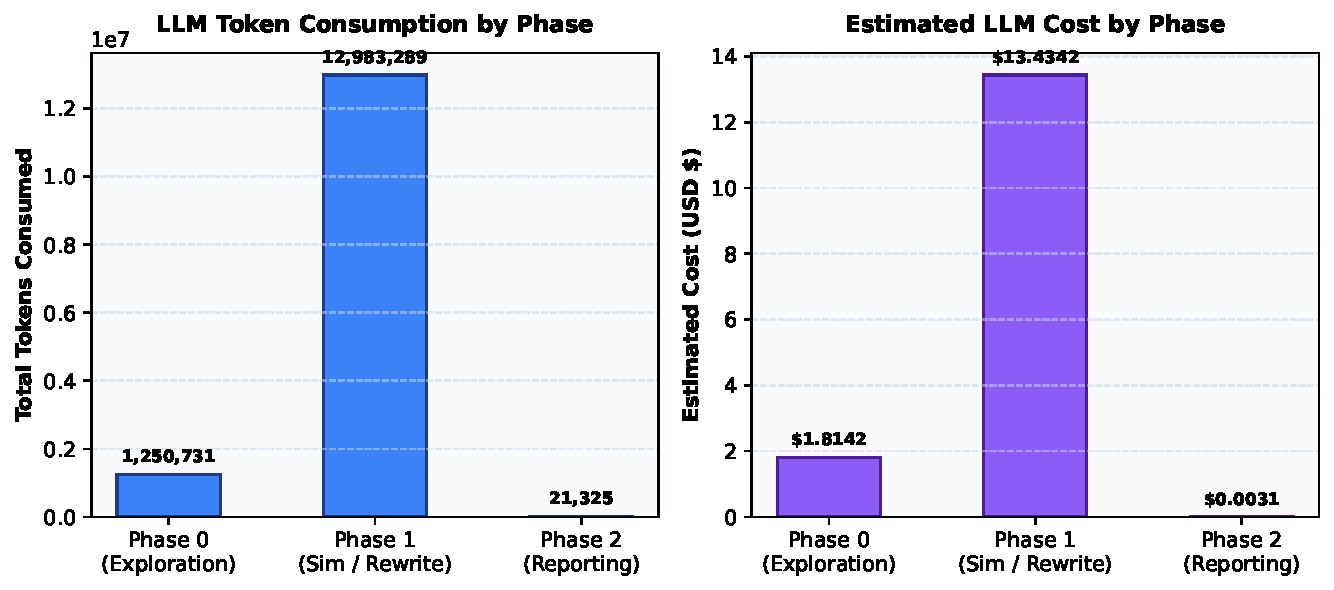
\includegraphics[width=0.95\linewidth]{figures/token_cost_summary.pdf}
\caption{Swarm-wide LLM token consumption and estimated dollar cost breakdown across operational phases.}
\label{fig:tokens}
\end{figure}

\begin{table}[htbp]
\caption{Swarm-Wide LLM Token Consumption and Cost Audit}
\label{tab:token_cost}
\centering
\begin{tabular}{lrrrrr}
\toprule
\textbf{Swarm Phase} \ &  \textbf{Calls} \ &  \textbf{Prompt Tok.} \ &  \textbf{Compl. Tok.} \ &  \textbf{Total Tok.} \ &  \textbf{Cost (\$)} \\
\midrule
Phase 0 (Candidate Exploration) \ &  6 \ &  1,183,865 \ &  66,866 \ &  1,250,731 \ &  \$1.8142 \\
Phase 1 (Code Rewrite \& Simulation) \ &  46 \ &  12,199,242 \ &  784,047 \ &  12,983,289 \ &  \$13.4342 \\
Phase 2 (Auditing \& Final Reporting) \ &  1 \ &  14,625 \ &  6,700 \ &  21,325 \ &  \$0.0031 \\
\midrule
\textbf{Swarm Total} \ &  \textbf{53} \ &  \textbf{13,397,732} \ &  \textbf{857,613} \ &  \textbf{14,255,345} \ &  \textbf{\$15.2514} \\
\bottomrule
\end{tabular}
\end{table}

\section{Architectural Recommendations and Next Steps}
1. \textbf{Adaptive Simulation Profiling Cutoff}: Increase the wall-clock timeout for \texttt{node6\_phase1\_simulate\_profile} from 300.0s to 600.0s for stochastic L1 noise configurations, or scale the integration horizon adaptively ($T = 0.5$ during exploratory Phase 1) to prevent premature dropouts of complex noise models.
2. \textbf{Isolate Inner-Loop ODE Timing from Fixed Host Overheads}: Refactor latency benchmarking to differentiate between graph setup/memory allocation overhead and pure ODE step integration time. The current 2.78\% latency drop for a 44.4\% step reduction demonstrates that host dispatch masks numerical acceleration.
3. \textbf{Prune Compiler Rewriter Context Windows}: Optimize \texttt{node3\_phase1\_compiler\_rewriter} prompt construction by substituting full operator graph dumps with targeted differential AST patches. Reducing prompt sizes from ~375k to under 80k tokens per call will cut Phase 1 operational expenditure by over 65\%.
4. \textbf{Broaden Exploration into Sparse Crossbar Topologies}: Phase 0 proposals should break away from the dense regime (\texttt{sparsity\_ratio = 0.0}) and systematically evaluate structured 2:4 and random block sparsity (e.g., \texttt{sparsity\_ratio} $\in [0.3, 0.7]$) to determine whether coupling matrix sparsity breaks the latency plateau observed in 6,656-oscillator Kuramoto dynamics.

\section{Conclusion}
The empirical results established in this optimization run provide actionable trade-offs and guide subsequent silicon tape-out parameters and swarm exploration sweeps.

\end{document}
